\documentclass[]{article}
\usepackage[T1]{fontenc}
\usepackage{lmodern}
\usepackage{amssymb,amsmath}
\usepackage{ifxetex,ifluatex}
\usepackage{fixltx2e} % provides \textsubscript
% use upquote if available, for straight quotes in verbatim environments
\IfFileExists{upquote.sty}{\usepackage{upquote}}{}
\ifnum 0\ifxetex 1\fi\ifluatex 1\fi=0 % if pdftex
  \usepackage[utf8]{inputenc}
\else % if luatex or xelatex
  \ifxetex
    \usepackage{mathspec}
    \usepackage{xltxtra,xunicode}
  \else
    \usepackage{fontspec}
  \fi
  \defaultfontfeatures{Mapping=tex-text,Scale=MatchLowercase}
  \newcommand{\euro}{€}
\fi
% use microtype if available
\IfFileExists{microtype.sty}{\usepackage{microtype}}{}
\usepackage{color}
\usepackage{fancyvrb}
\newcommand{\VerbBar}{|}
\newcommand{\VERB}{\Verb[commandchars=\\\{\}]}
\DefineVerbatimEnvironment{Highlighting}{Verbatim}{commandchars=\\\{\}}
% Add ',fontsize=\small' for more characters per line
\usepackage{framed}
\definecolor{shadecolor}{RGB}{248,248,248}
\newenvironment{Shaded}{\begin{snugshade}}{\end{snugshade}}
\newcommand{\KeywordTok}[1]{\textcolor[rgb]{0.13,0.29,0.53}{\textbf{{#1}}}}
\newcommand{\DataTypeTok}[1]{\textcolor[rgb]{0.13,0.29,0.53}{{#1}}}
\newcommand{\DecValTok}[1]{\textcolor[rgb]{0.00,0.00,0.81}{{#1}}}
\newcommand{\BaseNTok}[1]{\textcolor[rgb]{0.00,0.00,0.81}{{#1}}}
\newcommand{\FloatTok}[1]{\textcolor[rgb]{0.00,0.00,0.81}{{#1}}}
\newcommand{\CharTok}[1]{\textcolor[rgb]{0.31,0.60,0.02}{{#1}}}
\newcommand{\StringTok}[1]{\textcolor[rgb]{0.31,0.60,0.02}{{#1}}}
\newcommand{\CommentTok}[1]{\textcolor[rgb]{0.56,0.35,0.01}{\textit{{#1}}}}
\newcommand{\OtherTok}[1]{\textcolor[rgb]{0.56,0.35,0.01}{{#1}}}
\newcommand{\AlertTok}[1]{\textcolor[rgb]{0.94,0.16,0.16}{{#1}}}
\newcommand{\FunctionTok}[1]{\textcolor[rgb]{0.00,0.00,0.00}{{#1}}}
\newcommand{\RegionMarkerTok}[1]{{#1}}
\newcommand{\ErrorTok}[1]{\textbf{{#1}}}
\newcommand{\NormalTok}[1]{{#1}}
\usepackage{graphicx}
% Redefine \includegraphics so that, unless explicit options are
% given, the image width will not exceed the width of the page.
% Images get their normal width if they fit onto the page, but
% are scaled down if they would overflow the margins.
\makeatletter
\def\ScaleIfNeeded{%
  \ifdim\Gin@nat@width>\linewidth
    \linewidth
  \else
    \Gin@nat@width
  \fi
}
\makeatother
\let\Oldincludegraphics\includegraphics
{%
 \catcode`\@=11\relax%
 \gdef\includegraphics{\@ifnextchar[{\Oldincludegraphics}{\Oldincludegraphics[width=\ScaleIfNeeded]}}%
}%
\ifxetex
  \usepackage[setpagesize=false, % page size defined by xetex
              unicode=false, % unicode breaks when used with xetex
              xetex]{hyperref}
\else
  \usepackage[unicode=true]{hyperref}
\fi
\hypersetup{breaklinks=true,
            bookmarks=true,
            pdfauthor={},
            pdftitle={},
            colorlinks=true,
            citecolor=blue,
            urlcolor=blue,
            linkcolor=magenta,
            pdfborder={0 0 0}}
\urlstyle{same}  % don't use monospace font for urls
\setlength{\parindent}{0pt}
\setlength{\parskip}{6pt plus 2pt minus 1pt}
\setlength{\emergencystretch}{3em}  % prevent overfull lines
\setcounter{secnumdepth}{0}

\author{}
\date{}

\begin{document}

\begin{Shaded}
\begin{Highlighting}[]
\KeywordTok{install.packages}\NormalTok{(}\StringTok{"ape"}\NormalTok{)}
\end{Highlighting}
\end{Shaded}

\begin{Shaded}
\begin{Highlighting}[]
\KeywordTok{library}\NormalTok{(ape)}
\end{Highlighting}
\end{Shaded}

\begin{Shaded}
\begin{Highlighting}[]
\NormalTok{primatedata <-}\StringTok{ }\KeywordTok{read.table}\NormalTok{(}\StringTok{"Primatedata.txt"}\NormalTok{, }\DataTypeTok{sep =} \StringTok{"}\CharTok{\textbackslash{}t}\StringTok{"}\NormalTok{, }\DataTypeTok{header =} \OtherTok{TRUE}\NormalTok{)}
\end{Highlighting}
\end{Shaded}

\begin{Shaded}
\begin{Highlighting}[]
\KeywordTok{str}\NormalTok{(primatedata)}
\end{Highlighting}
\end{Shaded}

\begin{verbatim}
## 'data.frame':    77 obs. of  8 variables:
##  $ Order          : Factor w/ 1 level "Primates": 1 1 1 1 1 1 1 1 1 1 ...
##  $ Family         : Factor w/ 15 levels "Aotidae","Atelidae",..: 2 2 2 14 3 3 3 4 4 4 ...
##  $ Binomial       : Factor w/ 77 levels "Alouatta palliata",..: 5 6 7 8 9 10 11 15 16 17 ...
##  $ AdultBodyMass_g: num  6692 7582 8697 958 558 ...
##  $ GestationLen_d : num  138 226 228 164 154 ...
##  $ HomeRange_km2  : num  2.28 0.73 1.36 0.02 0.32 0.02 0.00212 0.51 0.16 0.24 ...
##  $ MaxLongevity_m : num  336 328 454 304 215 ...
##  $ SocialGroupSize: num  14.5 42 20 2.95 6.85 ...
\end{verbatim}

\begin{Shaded}
\begin{Highlighting}[]
\KeywordTok{head}\NormalTok{(primatedata)}
\end{Highlighting}
\end{Shaded}

\begin{verbatim}
##      Order      Family           Binomial AdultBodyMass_g GestationLen_d
## 1 Primates    Atelidae   Ateles belzebuth          6692.4          138.2
## 2 Primates    Atelidae   Ateles geoffroyi          7582.4          226.4
## 3 Primates    Atelidae    Ateles paniscus          8697.2          228.2
## 4 Primates Pitheciidae  Callicebus moloch           958.1          164.0
## 5 Primates     Cebidae  Callimico goeldii           558.0          154.0
## 6 Primates     Cebidae Callithrix jacchus           290.2          144.0
##   HomeRange_km2 MaxLongevity_m SocialGroupSize
## 1          2.28          336.0           14.50
## 2          0.73          327.6           42.00
## 3          1.36          453.6           20.00
## 4          0.02          303.6            2.95
## 5          0.32          214.8            6.85
## 6          0.02          201.6            8.55
\end{verbatim}

\begin{Shaded}
\begin{Highlighting}[]
\KeywordTok{names}\NormalTok{(primatedata)}
\end{Highlighting}
\end{Shaded}

\begin{verbatim}
## [1] "Order"           "Family"          "Binomial"        "AdultBodyMass_g"
## [5] "GestationLen_d"  "HomeRange_km2"   "MaxLongevity_m"  "SocialGroupSize"
\end{verbatim}

This gives you the names of the columns.

\begin{Shaded}
\begin{Highlighting}[]
\NormalTok{primatedata}
\end{Highlighting}
\end{Shaded}

\begin{Shaded}
\begin{Highlighting}[]
\NormalTok{primatetree <-}\StringTok{ }\KeywordTok{read.nexus}\NormalTok{(}\StringTok{"consensusTree_10kTrees_Version2.nex"}\NormalTok{)}
\end{Highlighting}
\end{Shaded}

Let's examine the tree by typing:

\begin{Shaded}
\begin{Highlighting}[]
\NormalTok{primatetree}
\end{Highlighting}
\end{Shaded}

\begin{verbatim}
## 
## Phylogenetic tree with 226 tips and 221 internal nodes.
## 
## Tip labels:
##  Allenopithecus_nigroviridis, Cercopithecus_ascanius, Cercopithecus_cephus, Cercopithecus_cephus_cephus, Cercopithecus_cephus_ngottoensis, Cercopithecus_diana, ...
## 
## Rooted; includes branch lengths.
\end{verbatim}

\begin{Shaded}
\begin{Highlighting}[]
\KeywordTok{str}\NormalTok{(primatetree)}
\end{Highlighting}
\end{Shaded}

\begin{verbatim}
## List of 4
##  $ edge       : int [1:446, 1:2] 227 228 229 230 231 232 233 234 234 235 ...
##  $ edge.length: num [1:446] 4.95 17.69 19.65 8.12 4.82 ...
##  $ Nnode      : int 221
##  $ tip.label  : chr [1:226] "Allenopithecus_nigroviridis" "Cercopithecus_ascanius" "Cercopithecus_cephus" "Cercopithecus_cephus_cephus" ...
##  - attr(*, "class")= chr "phylo"
##  - attr(*, "order")= chr "cladewise"
\end{verbatim}

\begin{Shaded}
\begin{Highlighting}[]
\KeywordTok{plot}\NormalTok{(primatetree)}
\end{Highlighting}
\end{Shaded}

\begin{Shaded}
\begin{Highlighting}[]
\KeywordTok{plot}\NormalTok{(primatetree, }\DataTypeTok{cex =} \FloatTok{0.5}\NormalTok{)}
\end{Highlighting}
\end{Shaded}

\begin{Shaded}
\begin{Highlighting}[]
\KeywordTok{zoom}\NormalTok{(primatetree, }\KeywordTok{list}\NormalTok{(}\KeywordTok{grep}\NormalTok{(}\StringTok{"Cercopithecus"}\NormalTok{, primatetree\$tip.label)), }
\DataTypeTok{subtree =} \OtherTok{FALSE}\NormalTok{)}
\end{Highlighting}
\end{Shaded}

\begin{Shaded}
\begin{Highlighting}[]
\KeywordTok{zoom}\NormalTok{(primatetree, }\KeywordTok{list}\NormalTok{(}\KeywordTok{grep}\NormalTok{(}\StringTok{"Cercopithecus"}\NormalTok{, primatetree\$tip.label)), }\DataTypeTok{subtree =} \OtherTok{TRUE}\NormalTok{)}
\end{Highlighting}
\end{Shaded}

\begin{Shaded}
\begin{Highlighting}[]
\NormalTok{primatetree2 <-}\StringTok{ }\KeywordTok{drop.tip}\NormalTok{(primatetree, }\StringTok{"Aotus_azarae_infulatus"}\NormalTok{)}
\KeywordTok{str}\NormalTok{(primatetree2)}
\end{Highlighting}
\end{Shaded}

\begin{verbatim}
## List of 4
##  $ edge       : int [1:444, 1:2] 226 227 228 229 230 231 232 233 233 234 ...
##  $ edge.length: num [1:444] 4.95 17.69 19.65 8.12 4.82 ...
##  $ Nnode      : int 220
##  $ tip.label  : chr [1:225] "Allenopithecus_nigroviridis" "Cercopithecus_ascanius" "Cercopithecus_cephus" "Cercopithecus_cephus_cephus" ...
##  - attr(*, "class")= chr "phylo"
##  - attr(*, "order")= chr "cladewise"
\end{verbatim}

\begin{Shaded}
\begin{Highlighting}[]
\StringTok{`}\DataTypeTok{?}\StringTok{`}\NormalTok{(plot.phylo)}
\end{Highlighting}
\end{Shaded}

\begin{Shaded}
\begin{Highlighting}[]
\KeywordTok{par}\NormalTok{(}\DataTypeTok{mfrow =} \KeywordTok{c}\NormalTok{(}\DecValTok{1}\NormalTok{, }\DecValTok{1}\NormalTok{))}
\KeywordTok{plot}\NormalTok{(primatetree, }\DataTypeTok{type =} \StringTok{"fan"}\NormalTok{, }\DataTypeTok{edge.color =} \StringTok{"deeppink"}\NormalTok{, }\DataTypeTok{tip.color =} \StringTok{"green"}\NormalTok{, }
    \DataTypeTok{cex =} \FloatTok{0.5}\NormalTok{)}
\end{Highlighting}
\end{Shaded}

\begin{Shaded}
\begin{Highlighting}[]
\KeywordTok{plot}\NormalTok{(primatetree)}
\KeywordTok{axisPhylo}\NormalTok{()}
\end{Highlighting}
\end{Shaded}

\begin{Shaded}
\begin{Highlighting}[]
\KeywordTok{is.binary.tree}\NormalTok{(primatetree)  }\CommentTok{# we want this to be TRUE}
\end{Highlighting}
\end{Shaded}

\begin{verbatim}
## [1] FALSE
\end{verbatim}

\begin{Shaded}
\begin{Highlighting}[]
\NormalTok{primatetree <-}\StringTok{ }\KeywordTok{multi2di}\NormalTok{(primatetree)}
\end{Highlighting}
\end{Shaded}

\begin{Shaded}
\begin{Highlighting}[]
\NormalTok{primatetree.reroot <-}\StringTok{ }\KeywordTok{root}\NormalTok{(primatetree, }\StringTok{"Saimiri_sciureus"}\NormalTok{)}
\KeywordTok{plot}\NormalTok{(primatetree.reroot)}
\end{Highlighting}
\end{Shaded}

\begin{Shaded}
\begin{Highlighting}[]
\NormalTok{primatedata\$Binomial <-}\StringTok{ }\KeywordTok{gsub}\NormalTok{(}\StringTok{" "}\NormalTok{, }\StringTok{"_"}\NormalTok{, primatedata\$Binomial)}
\end{Highlighting}
\end{Shaded}

\begin{Shaded}
\begin{Highlighting}[]
\KeywordTok{row.names}\NormalTok{(primatedata) <-}\StringTok{ }\NormalTok{primatedata\$Binomial}
\end{Highlighting}
\end{Shaded}

\begin{Shaded}
\begin{Highlighting}[]
\KeywordTok{par}\NormalTok{(}\DataTypeTok{mfrow =} \KeywordTok{c}\NormalTok{(}\DecValTok{2}\NormalTok{, }\DecValTok{2}\NormalTok{))}
\end{Highlighting}
\end{Shaded}

\begin{Shaded}
\begin{Highlighting}[]
\KeywordTok{hist}\NormalTok{(primatedata\$AdultBodyMass_g)}
\KeywordTok{hist}\NormalTok{(primatedata\$GestationLen_d)}
\end{Highlighting}
\end{Shaded}

\begin{Shaded}
\begin{Highlighting}[]
\KeywordTok{hist}\NormalTok{(}\KeywordTok{log}\NormalTok{(primatedata\$AdultBodyMass_g))}
\KeywordTok{hist}\NormalTok{(}\KeywordTok{log}\NormalTok{(primatedata\$GestationLen_d))}
\end{Highlighting}
\end{Shaded}

\begin{Shaded}
\begin{Highlighting}[]
\KeywordTok{hist}\NormalTok{(}\KeywordTok{log}\NormalTok{(primatedata\$GestationLen_d), }\DataTypeTok{col =} \KeywordTok{rainbow}\NormalTok{(}\DecValTok{8}\NormalTok{))}
\end{Highlighting}
\end{Shaded}

\begin{figure}[htbp]
\centering
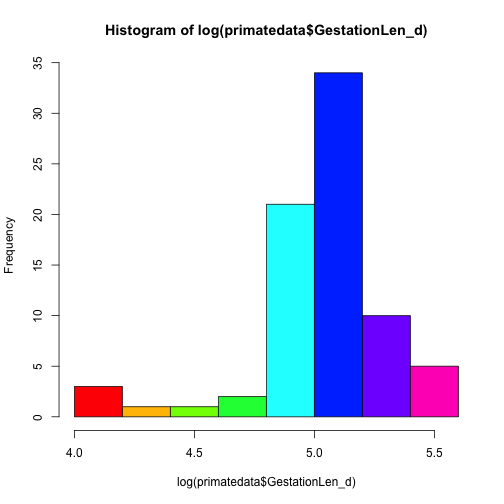
\includegraphics{figure/unnamed-chunk-25.png}
\caption{plot of chunk unnamed-chunk-25}
\end{figure}

\begin{Shaded}
\begin{Highlighting}[]
\KeywordTok{par}\NormalTok{(}\DataTypeTok{mfrow =} \KeywordTok{c}\NormalTok{(}\DecValTok{1}\NormalTok{, }\DecValTok{1}\NormalTok{))}
\end{Highlighting}
\end{Shaded}

\begin{Shaded}
\begin{Highlighting}[]
\NormalTok{model.ols <-}\StringTok{ }\KeywordTok{lm}\NormalTok{(}\KeywordTok{log}\NormalTok{(GestationLen_d) ~}\StringTok{ }\KeywordTok{log}\NormalTok{(AdultBodyMass_g), }\DataTypeTok{data =} \NormalTok{primatedata)}
\KeywordTok{summary}\NormalTok{(model.ols)}
\end{Highlighting}
\end{Shaded}

\begin{verbatim}
## 
## Call:
## lm(formula = log(GestationLen_d) ~ log(AdultBodyMass_g), data = primatedata)
## 
## Residuals:
##     Min      1Q  Median      3Q     Max 
## -0.6161 -0.0828  0.0065  0.1141  0.5056 
## 
## Coefficients:
##                      Estimate Std. Error t value Pr(>|t|)    
## (Intercept)            4.1038     0.1108   37.04  < 2e-16 ***
## log(AdultBodyMass_g)   0.1204     0.0141    8.54  1.1e-12 ***
## ---
## Signif. codes:  0 '***' 0.001 '**' 0.01 '*' 0.05 '.' 0.1 ' ' 1
## 
## Residual standard error: 0.198 on 75 degrees of freedom
## Multiple R-squared:  0.493,  Adjusted R-squared:  0.487 
## F-statistic:   73 on 1 and 75 DF,  p-value: 1.1e-12
\end{verbatim}

\begin{Shaded}
\begin{Highlighting}[]
\KeywordTok{plot}\NormalTok{(}\KeywordTok{log}\NormalTok{(GestationLen_d) ~}\StringTok{ }\KeywordTok{log}\NormalTok{(AdultBodyMass_g), }\DataTypeTok{data =} \NormalTok{primatedata)}
\KeywordTok{abline}\NormalTok{(model.ols)}
\end{Highlighting}
\end{Shaded}

\begin{Shaded}
\begin{Highlighting}[]
\KeywordTok{points}\NormalTok{(}\KeywordTok{log}\NormalTok{(GestationLen_d[Family ==}\StringTok{ "Cercopithecidae"}\NormalTok{]) ~}\StringTok{ }\KeywordTok{log}\NormalTok{(AdultBodyMass_g[Family ==}\StringTok{ }
\StringTok{    "Cercopithecidae"}\NormalTok{]), }\DataTypeTok{data =} \NormalTok{primatedata, }\DataTypeTok{col =} \StringTok{"blue"}\NormalTok{, }\DataTypeTok{pch =} \DecValTok{16}\NormalTok{)}
\end{Highlighting}
\end{Shaded}

\begin{Shaded}
\begin{Highlighting}[]
\NormalTok{primate <-}\StringTok{ }\KeywordTok{comparative.data}\NormalTok{(}\DataTypeTok{phy =} \NormalTok{primatetree, }\DataTypeTok{data =} \NormalTok{primatedata, }\DataTypeTok{names.col =} \NormalTok{Binomial, }
    \DataTypeTok{vcv =} \OtherTok{TRUE}\NormalTok{, }\DataTypeTok{na.omit =} \OtherTok{FALSE}\NormalTok{, }\DataTypeTok{warn.dropped =} \OtherTok{TRUE}\NormalTok{)}
\end{Highlighting}
\end{Shaded}

\begin{verbatim}
## Warning: Data dropped in compiling comparative data object
\end{verbatim}

\begin{Shaded}
\begin{Highlighting}[]
\NormalTok{primate$dropped$tips}
\end{Highlighting}
\end{Shaded}

\begin{verbatim}
##   [1] "Allenopithecus_nigroviridis"                  
##   [2] "Cercopithecus_cephus_cephus"                  
##   [3] "Cercopithecus_cephus_ngottoensis"             
##   [4] "Cercopithecus_diana"                          
##   [5] "Cercopithecus_erythrogaster_erythrogaster"    
##   [6] "Cercopithecus_erythrotis"                     
##   [7] "Cercopithecus_hamlyni"                        
##   [8] "Cercopithecus_lhoesti"                        
##   [9] "Cercopithecus_lowei"                          
##  [10] "Cercopithecus_mona"                           
##  [11] "Cercopithecus_petaurista"                     
##  [12] "Cercopithecus_preussi"                        
##  [13] "Cercopithecus_solatus"                        
##  [14] "Cercopithecus_wolfi"                          
##  [15] "Chlorocebus_aethiops"                         
##  [16] "Chlorocebus_pygerythrus"                      
##  [17] "Chlorocebus_sabaeus"                          
##  [18] "Chlorocebus_tantalus"                         
##  [19] "Allocebus_trichotis"                          
##  [20] "Avahi_laniger"                                
##  [21] "Avahi_occidentalis"                           
##  [22] "Cheirogaleus_crossleyi"                       
##  [23] "Eulemur_albifrons"                            
##  [24] "Eulemur_albocollaris"                         
##  [25] "Eulemur_collaris"                             
##  [26] "Eulemur_macaco_flavifrons"                    
##  [27] "Eulemur_macaco_macaco"                        
##  [28] "Eulemur_rubriventer"                          
##  [29] "Eulemur_rufus"                                
##  [30] "Eulemur_sanfordi"                             
##  [31] "Hapalemur_alaotrensis"                        
##  [32] "Hapalemur_aureus"                             
##  [33] "Hapalemur_griseus_griseus"                    
##  [34] "Hapalemur_griseus_meridionalis"               
##  [35] "Hapalemur_occidentalis"                       
##  [36] "Indri_indri"                                  
##  [37] "Lepilemur_aeeclis"                            
##  [38] "Lepilemur_ankaranensis"                       
##  [39] "Lepilemur_dorsalis"                           
##  [40] "Lepilemur_edwardsi"                           
##  [41] "Lepilemur_microdon"                           
##  [42] "Lepilemur_mitsinjoensis"                      
##  [43] "Lepilemur_randrianasoli"                      
##  [44] "Lepilemur_ruficaudatus"                       
##  [45] "Lepilemur_sahamalazensis"                     
##  [46] "Lepilemur_seali"                              
##  [47] "Lepilemur_septentrionalis"                    
##  [48] "Microcebus_berthae"                           
##  [49] "Microcebus_bongolavensis"                     
##  [50] "Microcebus_danfossi"                          
##  [51] "Microcebus_griseorufus"                       
##  [52] "Microcebus_jollyae"                           
##  [53] "Microcebus_lehilahytsara"                     
##  [54] "Microcebus_lokobensis"                        
##  [55] "Microcebus_mittermeieri"                      
##  [56] "Microcebus_myoxinus"                          
##  [57] "Microcebus_ravelobensis"                      
##  [58] "Microcebus_sambiranensis"                     
##  [59] "Microcebus_simmonsi"                          
##  [60] "Microcebus_tavaratra"                         
##  [61] "Propithecus_coquereli"                        
##  [62] "Propithecus_diadema"                          
##  [63] "Propithecus_edwardsi"                         
##  [64] "Propithecus_tattersalli"                      
##  [65] "Varecia_rubra"                                
##  [66] "Varecia_variegata_variegata"                  
##  [67] "Alouatta_caraya"                              
##  [68] "Alouatta_sara"                                
##  [69] "Ateles_fusciceps"                             
##  [70] "Ateles_geoffroyi_ornatus"                     
##  [71] "Ateles_geoffroyi_vellerosus"                  
##  [72] "Brachyteles_arachnoides"                      
##  [73] "Aotus_azarae"                                 
##  [74] "Aotus_azarae_infulatus"                       
##  [75] "Aotus_lemurinus_griseimembra"                 
##  [76] "Aotus_nancymaae"                              
##  [77] "Callithrix_(Mico)_emiliae"                    
##  [78] "Callithrix_argentata"                         
##  [79] "Callithrix_aurita"                            
##  [80] "Callithrix_geoffroyi"                         
##  [81] "Callithrix_humeralifera"                      
##  [82] "Callithrix_kuhli"                             
##  [83] "Callithrix_penicillata"                       
##  [84] "Leontopithecus_chrysomelas"                   
##  [85] "Leontopithecus_chrysopygus"                   
##  [86] "Saguinus_geoffroyi"                           
##  [87] "Saguinus_imperator"                           
##  [88] "Saimiri_boliviensis_boliviensis"              
##  [89] "Saimiri_oerstedii"                            
##  [90] "Arctocebus_aureus"                            
##  [91] "Arctocebus_calabarensis"                      
##  [92] "Loris_lydekkerianus_grandis"                  
##  [93] "Loris_lydekkerianus_malabaricus"              
##  [94] "Nycticebus_coucang"                           
##  [95] "Nycticebus_pygmaeus"                          
##  [96] "Bunopithecus_hoolock"                         
##  [97] "Gorilla_gorilla_gorilla"                      
##  [98] "Homo_sapiens"                                 
##  [99] "Hylobates_agilis"                             
## [100] "Hylobates_klossii"                            
## [101] "Hylobates_moloch"                             
## [102] "Hylobates_muelleri"                           
## [103] "Nomascus_gabriellae"                          
## [104] "Nomascus_leucogenys"                          
## [105] "Pan_troglodytes_schweinfurthii"               
## [106] "Pan_troglodytes_troglodytes"                  
## [107] "Pan_troglodytes_verus"                        
## [108] "Pongo_abelii"                                 
## [109] "Pongo_pygmaeus_pygmaeus"                      
## [110] "Callicebus_donacophilus"                      
## [111] "Cercocebus_agilis"                            
## [112] "Cercocebus_atys"                              
## [113] "Cercocebus_torquatus"                         
## [114] "Lophocebus_aterrimus"                         
## [115] "Macaca_arctoides"                             
## [116] "Macaca_assamensis"                            
## [117] "Macaca_cyclopis"                              
## [118] "Macaca_hecki"                                 
## [119] "Macaca_leonina"                               
## [120] "Macaca_maura"                                 
## [121] "Macaca_nigra"                                 
## [122] "Macaca_nigrescens"                            
## [123] "Macaca_ochreata"                              
## [124] "Macaca_ochreata_brunnescens"                  
## [125] "Macaca_pagensis"                              
## [126] "Macaca_siberu"                                
## [127] "Macaca_thibetana"                             
## [128] "Macaca_tonkeana"                              
## [129] "Mandrillus_leucophaeus"                       
## [130] "Papio_papio"                                  
## [131] "Rungwecebus_kipunji"                          
## [132] "Colobus_angolensis"                           
## [133] "Piliocolobus_badius"                          
## [134] "Presbytis_melalophos"                         
## [135] "Pygathrix_nemaeus"                            
## [136] "Rhinopithecus_avunculus"                      
## [137] "Rhinopithecus_bieti"                          
## [138] "Rhinopithecus_brelichi"                       
## [139] "Rhinopithecus_roxellana"                      
## [140] "Trachypithecus_(Trachypithecus)_auratus"      
## [141] "Trachypithecus_(Trachypithecus)_poliocephalus"
## [142] "Trachypithecus_cristatus"                     
## [143] "Trachypithecus_francoisi"                     
## [144] "Trachypithecus_johnii"                        
## [145] "Trachypithecus_phayrei"                       
## [146] "Trachypithecus_pileatus"                      
## [147] "Euoticus_elegantulus"                         
## [148] "Galago_gallarum"                              
## [149] "Galago_zanzibaricus"
\end{verbatim}

\begin{Shaded}
\begin{Highlighting}[]
\NormalTok{primate$dropped$unmatched.rows}
\end{Highlighting}
\end{Shaded}

\begin{verbatim}
## character(0)
\end{verbatim}

\begin{Shaded}
\begin{Highlighting}[]
\NormalTok{model.pgls <-}\StringTok{ }\KeywordTok{pgls}\NormalTok{(}\KeywordTok{log}\NormalTok{(GestationLen_d) ~}\StringTok{ }\KeywordTok{log}\NormalTok{(AdultBodyMass_g), }\DataTypeTok{data =} \NormalTok{primate, }
    \DataTypeTok{lambda =} \StringTok{"ML"}\NormalTok{)}
\KeywordTok{summary}\NormalTok{(model.pgls)}
\end{Highlighting}
\end{Shaded}

\begin{verbatim}
## 
## Call:
## pgls(formula = log(GestationLen_d) ~ log(AdultBodyMass_g), data = primate, 
##     lambda = "ML")
## 
## Residuals:
##      Min       1Q   Median       3Q      Max 
## -0.09890 -0.01166  0.00308  0.01776  0.07513 
## 
## Branch length transformations:
## 
## kappa  [Fix]  : 1.000
## lambda [ ML]  : 0.892
##    lower bound : 0.000, p = 1.1e-14
##    upper bound : 1.000, p = 0.00046
##    95.0% CI   : (0.753, 0.967)
## delta  [Fix]  : 1.000
## 
## Coefficients:
##                      Estimate Std. Error t value Pr(>|t|)    
## (Intercept)            4.2902     0.1604   26.75  < 2e-16 ***
## log(AdultBodyMass_g)   0.1049     0.0196    5.34  9.5e-07 ***
## ---
## Signif. codes:  0 '***' 0.001 '**' 0.01 '*' 0.05 '.' 0.1 ' ' 1
## 
## Residual standard error: 0.0261 on 75 degrees of freedom
## Multiple R-squared: 0.276,   Adjusted R-squared: 0.266 
## F-statistic: 28.5 on 1 and 75 DF,  p-value: 9.48e-07
\end{verbatim}

\begin{Shaded}
\begin{Highlighting}[]
\KeywordTok{plot}\NormalTok{(}\KeywordTok{log}\NormalTok{(GestationLen_d) ~}\StringTok{ }\KeywordTok{log}\NormalTok{(AdultBodyMass_g), }\DataTypeTok{data =} \NormalTok{primate$data)}
\KeywordTok{abline}\NormalTok{(model.pgls)}
\end{Highlighting}
\end{Shaded}

\begin{Shaded}
\begin{Highlighting}[]
\NormalTok{model.pgls2 <-}\StringTok{ }\KeywordTok{pgls}\NormalTok{(}\KeywordTok{log}\NormalTok{(GestationLen_d) ~}\StringTok{ }\KeywordTok{log}\NormalTok{(AdultBodyMass_g), }\DataTypeTok{data =} \NormalTok{primate, }
    \DataTypeTok{lambda =} \StringTok{"ML"}\NormalTok{, }\DataTypeTok{bounds =} \KeywordTok{list}\NormalTok{(}\DataTypeTok{lambda =} \KeywordTok{c}\NormalTok{(}\FloatTok{1e-06}\NormalTok{, }\DecValTok{1}\NormalTok{)))}
\KeywordTok{summary}\NormalTok{(model.pgls2)}
\end{Highlighting}
\end{Shaded}

\begin{verbatim}
## 
## Call:
## pgls(formula = log(GestationLen_d) ~ log(AdultBodyMass_g), data = primate, 
##     lambda = "ML", bounds = list(lambda = c(1e-06, 1)))
## 
## Residuals:
##      Min       1Q   Median       3Q      Max 
## -0.09890 -0.01166  0.00308  0.01776  0.07513 
## 
## Branch length transformations:
## 
## kappa  [Fix]  : 1.000
## lambda [ ML]  : 0.892
##    lower bound : 0.000, p = 1.1e-14
##    upper bound : 1.000, p = 0.00046
##    95.0% CI   : (0.753, 0.967)
## delta  [Fix]  : 1.000
## 
## Coefficients:
##                      Estimate Std. Error t value Pr(>|t|)    
## (Intercept)            4.2902     0.1604   26.75  < 2e-16 ***
## log(AdultBodyMass_g)   0.1049     0.0196    5.34  9.5e-07 ***
## ---
## Signif. codes:  0 '***' 0.001 '**' 0.01 '*' 0.05 '.' 0.1 ' ' 1
## 
## Residual standard error: 0.0261 on 75 degrees of freedom
## Multiple R-squared: 0.276,   Adjusted R-squared: 0.266 
## F-statistic: 28.5 on 1 and 75 DF,  p-value: 9.48e-07
\end{verbatim}

\begin{Shaded}
\begin{Highlighting}[]
\NormalTok{lambda.profile <-}\StringTok{ }\KeywordTok{pgls.profile}\NormalTok{(model.pgls, }\StringTok{"lambda"}\NormalTok{)}
\KeywordTok{plot}\NormalTok{(lambda.profile)}
\end{Highlighting}
\end{Shaded}

\begin{Shaded}
\begin{Highlighting}[]
\KeywordTok{pgls.confint}\NormalTok{(model.pgls, }\StringTok{"lambda"}\NormalTok{)}
\end{Highlighting}
\end{Shaded}

\begin{verbatim}
## $opt
## lambda 
##  0.892 
## 
## $bounds.val
## [1] 1e-06 1e+00
## 
## $bounds.p
## [1] 1.144e-14 4.639e-04
## 
## $ci.val
## [1] 0.7534 0.9665
## 
## $ci
## [1] 0.95
\end{verbatim}

\begin{Shaded}
\begin{Highlighting}[]
\NormalTok{est.lambda <-}\StringTok{ }\KeywordTok{pgls}\NormalTok{(}\KeywordTok{log}\NormalTok{(GestationLen_d) ~}\StringTok{ }\DecValTok{1}\NormalTok{, }\DataTypeTok{data =} \NormalTok{primate, }\DataTypeTok{lambda =} \StringTok{"ML"}\NormalTok{)}
\KeywordTok{summary}\NormalTok{(est.lambda)}
\end{Highlighting}
\end{Shaded}

\begin{verbatim}
## 
## Call:
## pgls(formula = log(GestationLen_d) ~ 1, data = primate, lambda = "ML")
## 
## Residuals:
##      Min       1Q   Median       3Q      Max 
## -0.12835 -0.01446  0.00139  0.01757  0.07433 
## 
## Branch length transformations:
## 
## kappa  [Fix]  : 1.000
## lambda [ ML]  : 0.948
##    lower bound : 0.000, p = <2e-16
##    upper bound : 1.000, p = 0.03 
##    95.0% CI   : (0.859, 0.996)
## delta  [Fix]  : 1.000
## 
## Coefficients:
##             Estimate Std. Error t value Pr(>|t|)    
## (Intercept)    5.005      0.117    42.7   <2e-16 ***
## ---
## Signif. codes:  0 '***' 0.001 '**' 0.01 '*' 0.05 '.' 0.1 ' ' 1
## 
## Residual standard error: 0.0334 on 76 degrees of freedom
## Multiple R-squared:    0,    Adjusted R-squared:    0 
## F-statistic:  NaN on 0 and 76 DF,  p-value: NA
\end{verbatim}

\begin{Shaded}
\begin{Highlighting}[]
\KeywordTok{par}\NormalTok{(}\DataTypeTok{mfrow =} \KeywordTok{c}\NormalTok{(}\DecValTok{2}\NormalTok{, }\DecValTok{2}\NormalTok{))}
\KeywordTok{plot}\NormalTok{(model.pgls)}
\end{Highlighting}
\end{Shaded}

\begin{Shaded}
\begin{Highlighting}[]
\NormalTok{pgls.residuals <-}\StringTok{ }\KeywordTok{residuals}\NormalTok{(model.pgls, }\DataTypeTok{phylo =} \OtherTok{TRUE}\NormalTok{)}
\end{Highlighting}
\end{Shaded}

\begin{Shaded}
\begin{Highlighting}[]
\NormalTok{std.residuals <-}\StringTok{ }\NormalTok{pgls.residuals/}\KeywordTok{sqrt}\NormalTok{(}\KeywordTok{var}\NormalTok{(pgls.residuals))[}\DecValTok{1}\NormalTok{]}
\end{Highlighting}
\end{Shaded}

\begin{Shaded}
\begin{Highlighting}[]
\KeywordTok{rownames}\NormalTok{(std.residuals) <-}\StringTok{ }\KeywordTok{rownames}\NormalTok{(model.pgls$residuals)}
\end{Highlighting}
\end{Shaded}

\begin{Shaded}
\begin{Highlighting}[]
\KeywordTok{rownames}\NormalTok{(std.residuals)[(}\KeywordTok{abs}\NormalTok{(std.residuals) >}\StringTok{ }\DecValTok{3}\NormalTok{)]}
\end{Highlighting}
\end{Shaded}

\begin{verbatim}
## [1] "Colobus_polykomos"
\end{verbatim}

\begin{Shaded}
\begin{Highlighting}[]
\NormalTok{primate.no.outliers <-}\StringTok{ }\NormalTok{primate[-}\KeywordTok{which}\NormalTok{(}\KeywordTok{abs}\NormalTok{(std.residuals) >}\StringTok{ }\DecValTok{3}\NormalTok{), ]}
\end{Highlighting}
\end{Shaded}

\begin{Shaded}
\begin{Highlighting}[]
\NormalTok{model.pgls.no.outliers <-}\StringTok{ }\KeywordTok{pgls}\NormalTok{(}\KeywordTok{log}\NormalTok{(GestationLen_d) ~}\StringTok{ }\KeywordTok{log}\NormalTok{(AdultBodyMass_g), }\DataTypeTok{data =} \NormalTok{primate.no.outliers, }
    \DataTypeTok{lambda =} \StringTok{"ML"}\NormalTok{)}
\KeywordTok{summary}\NormalTok{(model.pgls.no.outliers)}
\end{Highlighting}
\end{Shaded}

\begin{verbatim}
## 
## Call:
## pgls(formula = log(GestationLen_d) ~ log(AdultBodyMass_g), data = primate.no.outliers, 
##     lambda = "ML")
## 
## Residuals:
##      Min       1Q   Median       3Q      Max 
## -0.05639 -0.01371 -0.00222  0.01434  0.08514 
## 
## Branch length transformations:
## 
## kappa  [Fix]  : 1.000
## lambda [ ML]  : 0.889
##    lower bound : 0.000, p = 2.1e-14
##    upper bound : 1.000, p = 0.00039
##    95.0% CI   : (0.748, 0.965)
## delta  [Fix]  : 1.000
## 
## Coefficients:
##                      Estimate Std. Error t value Pr(>|t|)    
## (Intercept)            4.2892     0.1608   26.67   <2e-16 ***
## log(AdultBodyMass_g)   0.1050     0.0197    5.33    1e-06 ***
## ---
## Signif. codes:  0 '***' 0.001 '**' 0.01 '*' 0.05 '.' 0.1 ' ' 1
## 
## Residual standard error: 0.0262 on 74 degrees of freedom
## Multiple R-squared: 0.277,   Adjusted R-squared: 0.267 
## F-statistic: 28.4 on 1 and 74 DF,  p-value: 1.03e-06
\end{verbatim}

\begin{Shaded}
\begin{Highlighting}[]
\KeywordTok{par}\NormalTok{(}\DataTypeTok{mfrow =} \KeywordTok{c}\NormalTok{(}\DecValTok{2}\NormalTok{, }\DecValTok{2}\NormalTok{))}
\KeywordTok{plot}\NormalTok{(model.pgls.no.outliers)}
\end{Highlighting}
\end{Shaded}

\begin{Shaded}
\begin{Highlighting}[]
\NormalTok{lngest <-}\StringTok{ }\KeywordTok{log}\NormalTok{(primatedata$GestationLen_d)}
\KeywordTok{names}\NormalTok{(lngest) <-}\StringTok{ }\NormalTok{primatedata$Binomial}
\end{Highlighting}
\end{Shaded}

\begin{Shaded}
\begin{Highlighting}[]
\KeywordTok{Kcalc}\NormalTok{(lngest[primatetree$tip.label], primatetree)}
\end{Highlighting}
\end{Shaded}

\begin{verbatim}
## [1] "Dropping taxa from the data because they are not present in the phylogeny:"
## [1] NA
## [1] "Dropping tips from the tree because they are not present in the data:"
##   [1] "Allenopithecus_nigroviridis"                  
##   [2] "Cercopithecus_cephus_cephus"                  
##   [3] "Cercopithecus_cephus_ngottoensis"             
##   [4] "Cercopithecus_diana"                          
##   [5] "Cercopithecus_erythrogaster_erythrogaster"    
##   [6] "Cercopithecus_erythrotis"                     
##   [7] "Cercopithecus_hamlyni"                        
##   [8] "Cercopithecus_lhoesti"                        
##   [9] "Cercopithecus_lowei"                          
##  [10] "Cercopithecus_mona"                           
##  [11] "Cercopithecus_petaurista"                     
##  [12] "Cercopithecus_preussi"                        
##  [13] "Cercopithecus_solatus"                        
##  [14] "Cercopithecus_wolfi"                          
##  [15] "Chlorocebus_aethiops"                         
##  [16] "Chlorocebus_pygerythrus"                      
##  [17] "Chlorocebus_sabaeus"                          
##  [18] "Chlorocebus_tantalus"                         
##  [19] "Allocebus_trichotis"                          
##  [20] "Avahi_laniger"                                
##  [21] "Avahi_occidentalis"                           
##  [22] "Cheirogaleus_crossleyi"                       
##  [23] "Eulemur_albifrons"                            
##  [24] "Eulemur_albocollaris"                         
##  [25] "Eulemur_collaris"                             
##  [26] "Eulemur_macaco_flavifrons"                    
##  [27] "Eulemur_macaco_macaco"                        
##  [28] "Eulemur_rubriventer"                          
##  [29] "Eulemur_rufus"                                
##  [30] "Eulemur_sanfordi"                             
##  [31] "Hapalemur_alaotrensis"                        
##  [32] "Hapalemur_aureus"                             
##  [33] "Hapalemur_griseus_griseus"                    
##  [34] "Hapalemur_griseus_meridionalis"               
##  [35] "Hapalemur_occidentalis"                       
##  [36] "Indri_indri"                                  
##  [37] "Lepilemur_aeeclis"                            
##  [38] "Lepilemur_ankaranensis"                       
##  [39] "Lepilemur_dorsalis"                           
##  [40] "Lepilemur_edwardsi"                           
##  [41] "Lepilemur_microdon"                           
##  [42] "Lepilemur_mitsinjoensis"                      
##  [43] "Lepilemur_randrianasoli"                      
##  [44] "Lepilemur_ruficaudatus"                       
##  [45] "Lepilemur_sahamalazensis"                     
##  [46] "Lepilemur_seali"                              
##  [47] "Lepilemur_septentrionalis"                    
##  [48] "Microcebus_berthae"                           
##  [49] "Microcebus_bongolavensis"                     
##  [50] "Microcebus_danfossi"                          
##  [51] "Microcebus_griseorufus"                       
##  [52] "Microcebus_jollyae"                           
##  [53] "Microcebus_lehilahytsara"                     
##  [54] "Microcebus_lokobensis"                        
##  [55] "Microcebus_mittermeieri"                      
##  [56] "Microcebus_myoxinus"                          
##  [57] "Microcebus_ravelobensis"                      
##  [58] "Microcebus_sambiranensis"                     
##  [59] "Microcebus_simmonsi"                          
##  [60] "Microcebus_tavaratra"                         
##  [61] "Propithecus_coquereli"                        
##  [62] "Propithecus_diadema"                          
##  [63] "Propithecus_edwardsi"                         
##  [64] "Propithecus_tattersalli"                      
##  [65] "Varecia_rubra"                                
##  [66] "Varecia_variegata_variegata"                  
##  [67] "Alouatta_caraya"                              
##  [68] "Alouatta_sara"                                
##  [69] "Ateles_fusciceps"                             
##  [70] "Ateles_geoffroyi_ornatus"                     
##  [71] "Ateles_geoffroyi_vellerosus"                  
##  [72] "Brachyteles_arachnoides"                      
##  [73] "Aotus_azarae"                                 
##  [74] "Aotus_azarae_infulatus"                       
##  [75] "Aotus_lemurinus_griseimembra"                 
##  [76] "Aotus_nancymaae"                              
##  [77] "Callithrix_(Mico)_emiliae"                    
##  [78] "Callithrix_argentata"                         
##  [79] "Callithrix_aurita"                            
##  [80] "Callithrix_geoffroyi"                         
##  [81] "Callithrix_humeralifera"                      
##  [82] "Callithrix_kuhli"                             
##  [83] "Callithrix_penicillata"                       
##  [84] "Leontopithecus_chrysomelas"                   
##  [85] "Leontopithecus_chrysopygus"                   
##  [86] "Saguinus_geoffroyi"                           
##  [87] "Saguinus_imperator"                           
##  [88] "Saimiri_boliviensis_boliviensis"              
##  [89] "Saimiri_oerstedii"                            
##  [90] "Arctocebus_aureus"                            
##  [91] "Arctocebus_calabarensis"                      
##  [92] "Loris_lydekkerianus_grandis"                  
##  [93] "Loris_lydekkerianus_malabaricus"              
##  [94] "Nycticebus_coucang"                           
##  [95] "Nycticebus_pygmaeus"                          
##  [96] "Bunopithecus_hoolock"                         
##  [97] "Gorilla_gorilla_gorilla"                      
##  [98] "Homo_sapiens"                                 
##  [99] "Hylobates_agilis"                             
## [100] "Hylobates_klossii"                            
## [101] "Hylobates_moloch"                             
## [102] "Hylobates_muelleri"                           
## [103] "Nomascus_gabriellae"                          
## [104] "Nomascus_leucogenys"                          
## [105] "Pan_troglodytes_schweinfurthii"               
## [106] "Pan_troglodytes_troglodytes"                  
## [107] "Pan_troglodytes_verus"                        
## [108] "Pongo_abelii"                                 
## [109] "Pongo_pygmaeus_pygmaeus"                      
## [110] "Callicebus_donacophilus"                      
## [111] "Cercocebus_agilis"                            
## [112] "Cercocebus_atys"                              
## [113] "Cercocebus_torquatus"                         
## [114] "Lophocebus_aterrimus"                         
## [115] "Macaca_arctoides"                             
## [116] "Macaca_assamensis"                            
## [117] "Macaca_cyclopis"                              
## [118] "Macaca_hecki"                                 
## [119] "Macaca_leonina"                               
## [120] "Macaca_maura"                                 
## [121] "Macaca_nigra"                                 
## [122] "Macaca_nigrescens"                            
## [123] "Macaca_ochreata"                              
## [124] "Macaca_ochreata_brunnescens"                  
## [125] "Macaca_pagensis"                              
## [126] "Macaca_siberu"                                
## [127] "Macaca_thibetana"                             
## [128] "Macaca_tonkeana"                              
## [129] "Mandrillus_leucophaeus"                       
## [130] "Papio_papio"                                  
## [131] "Rungwecebus_kipunji"                          
## [132] "Colobus_angolensis"                           
## [133] "Piliocolobus_badius"                          
## [134] "Presbytis_melalophos"                         
## [135] "Pygathrix_nemaeus"                            
## [136] "Rhinopithecus_avunculus"                      
## [137] "Rhinopithecus_bieti"                          
## [138] "Rhinopithecus_brelichi"                       
## [139] "Rhinopithecus_roxellana"                      
## [140] "Trachypithecus_(Trachypithecus)_auratus"      
## [141] "Trachypithecus_(Trachypithecus)_poliocephalus"
## [142] "Trachypithecus_cristatus"                     
## [143] "Trachypithecus_francoisi"                     
## [144] "Trachypithecus_johnii"                        
## [145] "Trachypithecus_phayrei"                       
## [146] "Trachypithecus_pileatus"                      
## [147] "Euoticus_elegantulus"                         
## [148] "Galago_gallarum"                              
## [149] "Galago_zanzibaricus"
\end{verbatim}

\begin{verbatim}
##        [,1]
## [1,] 0.7758
\end{verbatim}

\begin{Shaded}
\begin{Highlighting}[]
\KeywordTok{phylosignal}\NormalTok{(lngest[primatetree$tip.label], primatetree, }\DataTypeTok{reps =} \DecValTok{1000}\NormalTok{)}
\end{Highlighting}
\end{Shaded}

\begin{verbatim}
## [1] "Dropping taxa from the data because they are not present in the phylogeny:"
## [1] NA
## [1] "Dropping tips from the tree because they are not present in the data:"
##   [1] "Allenopithecus_nigroviridis"                  
##   [2] "Cercopithecus_cephus_cephus"                  
##   [3] "Cercopithecus_cephus_ngottoensis"             
##   [4] "Cercopithecus_diana"                          
##   [5] "Cercopithecus_erythrogaster_erythrogaster"    
##   [6] "Cercopithecus_erythrotis"                     
##   [7] "Cercopithecus_hamlyni"                        
##   [8] "Cercopithecus_lhoesti"                        
##   [9] "Cercopithecus_lowei"                          
##  [10] "Cercopithecus_mona"                           
##  [11] "Cercopithecus_petaurista"                     
##  [12] "Cercopithecus_preussi"                        
##  [13] "Cercopithecus_solatus"                        
##  [14] "Cercopithecus_wolfi"                          
##  [15] "Chlorocebus_aethiops"                         
##  [16] "Chlorocebus_pygerythrus"                      
##  [17] "Chlorocebus_sabaeus"                          
##  [18] "Chlorocebus_tantalus"                         
##  [19] "Allocebus_trichotis"                          
##  [20] "Avahi_laniger"                                
##  [21] "Avahi_occidentalis"                           
##  [22] "Cheirogaleus_crossleyi"                       
##  [23] "Eulemur_albifrons"                            
##  [24] "Eulemur_albocollaris"                         
##  [25] "Eulemur_collaris"                             
##  [26] "Eulemur_macaco_flavifrons"                    
##  [27] "Eulemur_macaco_macaco"                        
##  [28] "Eulemur_rubriventer"                          
##  [29] "Eulemur_rufus"                                
##  [30] "Eulemur_sanfordi"                             
##  [31] "Hapalemur_alaotrensis"                        
##  [32] "Hapalemur_aureus"                             
##  [33] "Hapalemur_griseus_griseus"                    
##  [34] "Hapalemur_griseus_meridionalis"               
##  [35] "Hapalemur_occidentalis"                       
##  [36] "Indri_indri"                                  
##  [37] "Lepilemur_aeeclis"                            
##  [38] "Lepilemur_ankaranensis"                       
##  [39] "Lepilemur_dorsalis"                           
##  [40] "Lepilemur_edwardsi"                           
##  [41] "Lepilemur_microdon"                           
##  [42] "Lepilemur_mitsinjoensis"                      
##  [43] "Lepilemur_randrianasoli"                      
##  [44] "Lepilemur_ruficaudatus"                       
##  [45] "Lepilemur_sahamalazensis"                     
##  [46] "Lepilemur_seali"                              
##  [47] "Lepilemur_septentrionalis"                    
##  [48] "Microcebus_berthae"                           
##  [49] "Microcebus_bongolavensis"                     
##  [50] "Microcebus_danfossi"                          
##  [51] "Microcebus_griseorufus"                       
##  [52] "Microcebus_jollyae"                           
##  [53] "Microcebus_lehilahytsara"                     
##  [54] "Microcebus_lokobensis"                        
##  [55] "Microcebus_mittermeieri"                      
##  [56] "Microcebus_myoxinus"                          
##  [57] "Microcebus_ravelobensis"                      
##  [58] "Microcebus_sambiranensis"                     
##  [59] "Microcebus_simmonsi"                          
##  [60] "Microcebus_tavaratra"                         
##  [61] "Propithecus_coquereli"                        
##  [62] "Propithecus_diadema"                          
##  [63] "Propithecus_edwardsi"                         
##  [64] "Propithecus_tattersalli"                      
##  [65] "Varecia_rubra"                                
##  [66] "Varecia_variegata_variegata"                  
##  [67] "Alouatta_caraya"                              
##  [68] "Alouatta_sara"                                
##  [69] "Ateles_fusciceps"                             
##  [70] "Ateles_geoffroyi_ornatus"                     
##  [71] "Ateles_geoffroyi_vellerosus"                  
##  [72] "Brachyteles_arachnoides"                      
##  [73] "Aotus_azarae"                                 
##  [74] "Aotus_azarae_infulatus"                       
##  [75] "Aotus_lemurinus_griseimembra"                 
##  [76] "Aotus_nancymaae"                              
##  [77] "Callithrix_(Mico)_emiliae"                    
##  [78] "Callithrix_argentata"                         
##  [79] "Callithrix_aurita"                            
##  [80] "Callithrix_geoffroyi"                         
##  [81] "Callithrix_humeralifera"                      
##  [82] "Callithrix_kuhli"                             
##  [83] "Callithrix_penicillata"                       
##  [84] "Leontopithecus_chrysomelas"                   
##  [85] "Leontopithecus_chrysopygus"                   
##  [86] "Saguinus_geoffroyi"                           
##  [87] "Saguinus_imperator"                           
##  [88] "Saimiri_boliviensis_boliviensis"              
##  [89] "Saimiri_oerstedii"                            
##  [90] "Arctocebus_aureus"                            
##  [91] "Arctocebus_calabarensis"                      
##  [92] "Loris_lydekkerianus_grandis"                  
##  [93] "Loris_lydekkerianus_malabaricus"              
##  [94] "Nycticebus_coucang"                           
##  [95] "Nycticebus_pygmaeus"                          
##  [96] "Bunopithecus_hoolock"                         
##  [97] "Gorilla_gorilla_gorilla"                      
##  [98] "Homo_sapiens"                                 
##  [99] "Hylobates_agilis"                             
## [100] "Hylobates_klossii"                            
## [101] "Hylobates_moloch"                             
## [102] "Hylobates_muelleri"                           
## [103] "Nomascus_gabriellae"                          
## [104] "Nomascus_leucogenys"                          
## [105] "Pan_troglodytes_schweinfurthii"               
## [106] "Pan_troglodytes_troglodytes"                  
## [107] "Pan_troglodytes_verus"                        
## [108] "Pongo_abelii"                                 
## [109] "Pongo_pygmaeus_pygmaeus"                      
## [110] "Callicebus_donacophilus"                      
## [111] "Cercocebus_agilis"                            
## [112] "Cercocebus_atys"                              
## [113] "Cercocebus_torquatus"                         
## [114] "Lophocebus_aterrimus"                         
## [115] "Macaca_arctoides"                             
## [116] "Macaca_assamensis"                            
## [117] "Macaca_cyclopis"                              
## [118] "Macaca_hecki"                                 
## [119] "Macaca_leonina"                               
## [120] "Macaca_maura"                                 
## [121] "Macaca_nigra"                                 
## [122] "Macaca_nigrescens"                            
## [123] "Macaca_ochreata"                              
## [124] "Macaca_ochreata_brunnescens"                  
## [125] "Macaca_pagensis"                              
## [126] "Macaca_siberu"                                
## [127] "Macaca_thibetana"                             
## [128] "Macaca_tonkeana"                              
## [129] "Mandrillus_leucophaeus"                       
## [130] "Papio_papio"                                  
## [131] "Rungwecebus_kipunji"                          
## [132] "Colobus_angolensis"                           
## [133] "Piliocolobus_badius"                          
## [134] "Presbytis_melalophos"                         
## [135] "Pygathrix_nemaeus"                            
## [136] "Rhinopithecus_avunculus"                      
## [137] "Rhinopithecus_bieti"                          
## [138] "Rhinopithecus_brelichi"                       
## [139] "Rhinopithecus_roxellana"                      
## [140] "Trachypithecus_(Trachypithecus)_auratus"      
## [141] "Trachypithecus_(Trachypithecus)_poliocephalus"
## [142] "Trachypithecus_cristatus"                     
## [143] "Trachypithecus_francoisi"                     
## [144] "Trachypithecus_johnii"                        
## [145] "Trachypithecus_phayrei"                       
## [146] "Trachypithecus_pileatus"                      
## [147] "Euoticus_elegantulus"                         
## [148] "Galago_gallarum"                              
## [149] "Galago_zanzibaricus"
\end{verbatim}

\begin{verbatim}
##        K PIC.variance.obs PIC.variance.rnd.mean PIC.variance.P
## 1 0.7758         0.001661               0.01212       0.000999
##   PIC.variance.Z
## 1         -2.281
\end{verbatim}

\begin{Shaded}
\begin{Highlighting}[]
\KeywordTok{setdiff}\NormalTok{(primatetree$tip.label, primatedata$Binomial)}
\end{Highlighting}
\end{Shaded}

\begin{verbatim}
##   [1] "Allenopithecus_nigroviridis"                  
##   [2] "Cercopithecus_cephus_cephus"                  
##   [3] "Cercopithecus_cephus_ngottoensis"             
##   [4] "Cercopithecus_diana"                          
##   [5] "Cercopithecus_erythrogaster_erythrogaster"    
##   [6] "Cercopithecus_erythrotis"                     
##   [7] "Cercopithecus_hamlyni"                        
##   [8] "Cercopithecus_lhoesti"                        
##   [9] "Cercopithecus_lowei"                          
##  [10] "Cercopithecus_mona"                           
##  [11] "Cercopithecus_petaurista"                     
##  [12] "Cercopithecus_preussi"                        
##  [13] "Cercopithecus_solatus"                        
##  [14] "Cercopithecus_wolfi"                          
##  [15] "Chlorocebus_aethiops"                         
##  [16] "Chlorocebus_pygerythrus"                      
##  [17] "Chlorocebus_sabaeus"                          
##  [18] "Chlorocebus_tantalus"                         
##  [19] "Allocebus_trichotis"                          
##  [20] "Avahi_laniger"                                
##  [21] "Avahi_occidentalis"                           
##  [22] "Cheirogaleus_crossleyi"                       
##  [23] "Eulemur_albifrons"                            
##  [24] "Eulemur_albocollaris"                         
##  [25] "Eulemur_collaris"                             
##  [26] "Eulemur_macaco_flavifrons"                    
##  [27] "Eulemur_macaco_macaco"                        
##  [28] "Eulemur_rubriventer"                          
##  [29] "Eulemur_rufus"                                
##  [30] "Eulemur_sanfordi"                             
##  [31] "Hapalemur_alaotrensis"                        
##  [32] "Hapalemur_aureus"                             
##  [33] "Hapalemur_griseus_griseus"                    
##  [34] "Hapalemur_griseus_meridionalis"               
##  [35] "Hapalemur_occidentalis"                       
##  [36] "Indri_indri"                                  
##  [37] "Lepilemur_aeeclis"                            
##  [38] "Lepilemur_ankaranensis"                       
##  [39] "Lepilemur_dorsalis"                           
##  [40] "Lepilemur_edwardsi"                           
##  [41] "Lepilemur_microdon"                           
##  [42] "Lepilemur_mitsinjoensis"                      
##  [43] "Lepilemur_randrianasoli"                      
##  [44] "Lepilemur_ruficaudatus"                       
##  [45] "Lepilemur_sahamalazensis"                     
##  [46] "Lepilemur_seali"                              
##  [47] "Lepilemur_septentrionalis"                    
##  [48] "Microcebus_berthae"                           
##  [49] "Microcebus_bongolavensis"                     
##  [50] "Microcebus_danfossi"                          
##  [51] "Microcebus_griseorufus"                       
##  [52] "Microcebus_jollyae"                           
##  [53] "Microcebus_lehilahytsara"                     
##  [54] "Microcebus_lokobensis"                        
##  [55] "Microcebus_mittermeieri"                      
##  [56] "Microcebus_myoxinus"                          
##  [57] "Microcebus_ravelobensis"                      
##  [58] "Microcebus_sambiranensis"                     
##  [59] "Microcebus_simmonsi"                          
##  [60] "Microcebus_tavaratra"                         
##  [61] "Propithecus_coquereli"                        
##  [62] "Propithecus_diadema"                          
##  [63] "Propithecus_edwardsi"                         
##  [64] "Propithecus_tattersalli"                      
##  [65] "Varecia_rubra"                                
##  [66] "Varecia_variegata_variegata"                  
##  [67] "Alouatta_caraya"                              
##  [68] "Alouatta_sara"                                
##  [69] "Ateles_fusciceps"                             
##  [70] "Ateles_geoffroyi_ornatus"                     
##  [71] "Ateles_geoffroyi_vellerosus"                  
##  [72] "Brachyteles_arachnoides"                      
##  [73] "Aotus_azarae"                                 
##  [74] "Aotus_azarae_infulatus"                       
##  [75] "Aotus_lemurinus_griseimembra"                 
##  [76] "Aotus_nancymaae"                              
##  [77] "Callithrix_(Mico)_emiliae"                    
##  [78] "Callithrix_argentata"                         
##  [79] "Callithrix_aurita"                            
##  [80] "Callithrix_geoffroyi"                         
##  [81] "Callithrix_humeralifera"                      
##  [82] "Callithrix_kuhli"                             
##  [83] "Callithrix_penicillata"                       
##  [84] "Leontopithecus_chrysomelas"                   
##  [85] "Leontopithecus_chrysopygus"                   
##  [86] "Saguinus_geoffroyi"                           
##  [87] "Saguinus_imperator"                           
##  [88] "Saimiri_boliviensis_boliviensis"              
##  [89] "Saimiri_oerstedii"                            
##  [90] "Arctocebus_aureus"                            
##  [91] "Arctocebus_calabarensis"                      
##  [92] "Loris_lydekkerianus_grandis"                  
##  [93] "Loris_lydekkerianus_malabaricus"              
##  [94] "Nycticebus_coucang"                           
##  [95] "Nycticebus_pygmaeus"                          
##  [96] "Bunopithecus_hoolock"                         
##  [97] "Gorilla_gorilla_gorilla"                      
##  [98] "Homo_sapiens"                                 
##  [99] "Hylobates_agilis"                             
## [100] "Hylobates_klossii"                            
## [101] "Hylobates_moloch"                             
## [102] "Hylobates_muelleri"                           
## [103] "Nomascus_gabriellae"                          
## [104] "Nomascus_leucogenys"                          
## [105] "Pan_troglodytes_schweinfurthii"               
## [106] "Pan_troglodytes_troglodytes"                  
## [107] "Pan_troglodytes_verus"                        
## [108] "Pongo_abelii"                                 
## [109] "Pongo_pygmaeus_pygmaeus"                      
## [110] "Callicebus_donacophilus"                      
## [111] "Cercocebus_agilis"                            
## [112] "Cercocebus_atys"                              
## [113] "Cercocebus_torquatus"                         
## [114] "Lophocebus_aterrimus"                         
## [115] "Macaca_arctoides"                             
## [116] "Macaca_assamensis"                            
## [117] "Macaca_cyclopis"                              
## [118] "Macaca_hecki"                                 
## [119] "Macaca_leonina"                               
## [120] "Macaca_maura"                                 
## [121] "Macaca_nigra"                                 
## [122] "Macaca_nigrescens"                            
## [123] "Macaca_ochreata"                              
## [124] "Macaca_ochreata_brunnescens"                  
## [125] "Macaca_pagensis"                              
## [126] "Macaca_siberu"                                
## [127] "Macaca_thibetana"                             
## [128] "Macaca_tonkeana"                              
## [129] "Mandrillus_leucophaeus"                       
## [130] "Papio_papio"                                  
## [131] "Rungwecebus_kipunji"                          
## [132] "Colobus_angolensis"                           
## [133] "Piliocolobus_badius"                          
## [134] "Presbytis_melalophos"                         
## [135] "Pygathrix_nemaeus"                            
## [136] "Rhinopithecus_avunculus"                      
## [137] "Rhinopithecus_bieti"                          
## [138] "Rhinopithecus_brelichi"                       
## [139] "Rhinopithecus_roxellana"                      
## [140] "Trachypithecus_(Trachypithecus)_auratus"      
## [141] "Trachypithecus_(Trachypithecus)_poliocephalus"
## [142] "Trachypithecus_cristatus"                     
## [143] "Trachypithecus_francoisi"                     
## [144] "Trachypithecus_johnii"                        
## [145] "Trachypithecus_phayrei"                       
## [146] "Trachypithecus_pileatus"                      
## [147] "Euoticus_elegantulus"                         
## [148] "Galago_gallarum"                              
## [149] "Galago_zanzibaricus"
\end{verbatim}

\begin{Shaded}
\begin{Highlighting}[]
\NormalTok{primatetree2 <-}\StringTok{ }\KeywordTok{drop.tip}\NormalTok{(primatetree, }\KeywordTok{setdiff}\NormalTok{(primatetree$tip.label, primatedata$Binomial))}
\end{Highlighting}
\end{Shaded}

\begin{Shaded}
\begin{Highlighting}[]
\KeywordTok{setdiff}\NormalTok{(primatedata$Binomial, primatetree$tip.label)}
\end{Highlighting}
\end{Shaded}

\begin{verbatim}
## character(0)
\end{verbatim}

\begin{Shaded}
\begin{Highlighting}[]
\NormalTok{matches <-}\StringTok{ }\KeywordTok{match}\NormalTok{(primatedata$Binomial, primatetree2$tip.label, }\DataTypeTok{nomatch =} \DecValTok{0}\NormalTok{)}
\NormalTok{primatedata2 <-}\StringTok{ }\KeywordTok{subset}\NormalTok{(primatedata, matches !=}\StringTok{ }\DecValTok{0}\NormalTok{)}
\end{Highlighting}
\end{Shaded}

\begin{Shaded}
\begin{Highlighting}[]
\KeywordTok{str}\NormalTok{(primatedata2)}
\end{Highlighting}
\end{Shaded}

\begin{verbatim}
## 'data.frame':    77 obs. of  8 variables:
##  $ Order          : Factor w/ 1 level "Primates": 1 1 1 1 1 1 1 1 1 1 ...
##  $ Family         : Factor w/ 15 levels "Aotidae","Atelidae",..: 2 2 2 14 3 3 3 4 4 4 ...
##  $ Binomial       : chr  "Ateles_belzebuth" "Ateles_geoffroyi" "Ateles_paniscus" "Callicebus_moloch" ...
##  $ AdultBodyMass_g: num  6692 7582 8697 958 558 ...
##  $ GestationLen_d : num  138 226 228 164 154 ...
##  $ HomeRange_km2  : num  2.28 0.73 1.36 0.02 0.32 0.02 0.00212 0.51 0.16 0.24 ...
##  $ MaxLongevity_m : num  336 328 454 304 215 ...
##  $ SocialGroupSize: num  14.5 42 20 2.95 6.85 ...
\end{verbatim}

\begin{Shaded}
\begin{Highlighting}[]
\KeywordTok{str}\NormalTok{(primatetree2)}
\end{Highlighting}
\end{Shaded}

\begin{verbatim}
## List of 4
##  $ edge       : int [1:152, 1:2] 78 79 80 81 82 83 84 85 86 87 ...
##  $ edge.length: num [1:152] 4.95 17.69 19.65 8.12 4.82 ...
##  $ Nnode      : int 76
##  $ tip.label  : chr [1:77] "Cercopithecus_ascanius" "Cercopithecus_cephus" "Cercopithecus_mitis" "Cercopithecus_neglectus" ...
##  - attr(*, "class")= chr "phylo"
##  - attr(*, "order")= chr "cladewise"
\end{verbatim}

\end{document}
